\begin{figure}[t]
  \centering
  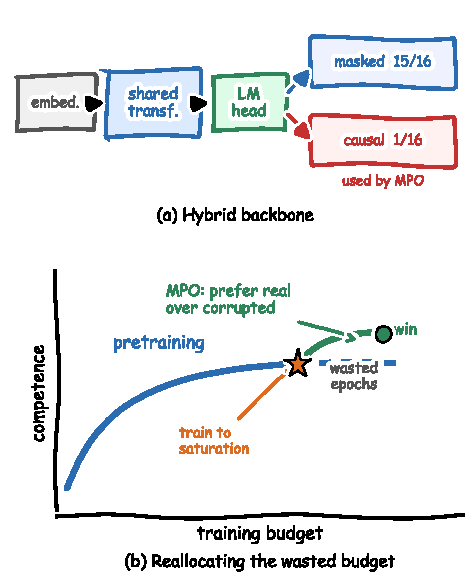
\includegraphics[width=0.86\columnwidth]{figures/fig_abstract}
  \caption{\textbf{The idea in one picture.} (a) The hybrid backbone: one shared
  transformer and a single language-model head, trained on both a masked
  objective ($15/16$ of batches) and a causal one ($1/16$). The causal mode is
  what \MPO{} later exploits. (b) Standard pretraining saturates, then wastes its
  final epochs (dashed). Starting from that saturation checkpoint, \MPO{} spends
  the leftover budget teaching the model to prefer real sentences over corrupted
  ones, and matches the fully-trained baseline in fewer epochs.}
  \label{fig:abstract}
\end{figure}
